\documentclass[a4spaper]{article}

\usepackage[english]{babel}
\usepackage[utf8]{inputenc}
\usepackage{amsmath}
\usepackage{graphicx}
\usepackage[colorinlistoftodos]{todonotes}
\usepackage{caption}
\usepackage{subcaption}
\usepackage{here}

\title{Computational Photography \\ Project 2, Fall 2014}

\author{Mich\`ele Wyss, 10-104-123}

\date{October 16, 2014}

\graphicspath{{imgs/}}
\begin{document}
\maketitle
\section{Tone Mapping using the Bilateral Filter}
\subsection*{The Bilateral Filter and its Parameters}
The main parameters that a user can set for the bilateral filter are the standard deviations $\sigma_s$ for the spatial and $\sigma_r$ for the range kernel. 
Both kernels are usually chosen to be Gaussians. 
Intuitively, $\sigma_s$ controls the {\em amount} of blurring, and $\sigma_r$ controls {\em what} is blurred. 
A small value of $\sigma_r$ means that already very small difference in intensity stop the averaging process. 
In this case, no matter how large $\sigma_s$ is, the image won't be smoothed because every little change in intensity will be interpreted as an edge and smoothing will be stopped by the edge-stopping function (range kernel). 
For an example, see Figure \ref{fig:jerry_small_range}. 
Higher values for $\sigma_r$ allow the filter to average pixels that are less similar to each other (see Figure \ref{fig:kernel_small_range}). 
However, in the case of a too high value for the standard deviation of the range filter kernel $\sigma_r$, the bilateral filter performs like a usual low-pass Gaussian filter (see Figure \ref{fig:jerry_large_range}). 
By finding appropriate values for the standard deviations, one can achieve smoothing of the image while preserving edges (see Figure \ref{fig:edge-preserving-smoothing}).
\begin{figure}[ht]
	%\centering
	\begin{subfigure}[h]{0.48\textwidth}
		\centering
		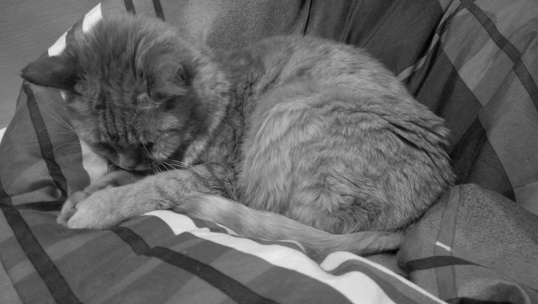
\includegraphics[width=\textwidth]{jerry_gray}
		\caption*{Input image}
	\end{subfigure}
	~
	\begin{subfigure}[h]{0.48\textwidth}
	  \centering
	  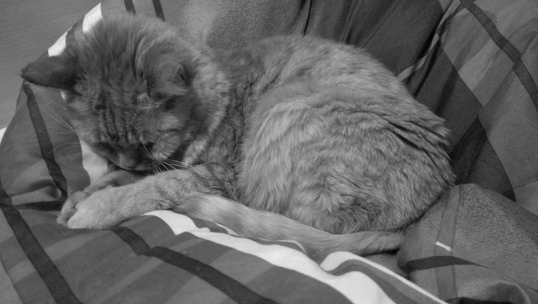
\includegraphics[width=\textwidth]{jerry_flt_1_0-001}
	  \caption*{$\sigma_s = 1, \sigma_r = 0.001$}
	\end{subfigure}
	
	\vspace{2mm}
	\begin{subfigure}[h]{0.48\textwidth}
		\centering
		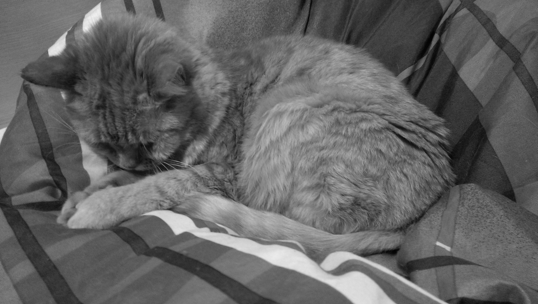
\includegraphics[width=\textwidth]{jerry_flt_10_0-001}
		\caption*{$\sigma_s = 10, \sigma_r = 0.001$}
	\end{subfigure}
	~
	\begin{subfigure}[h]{0.48\textwidth}
		\centering
		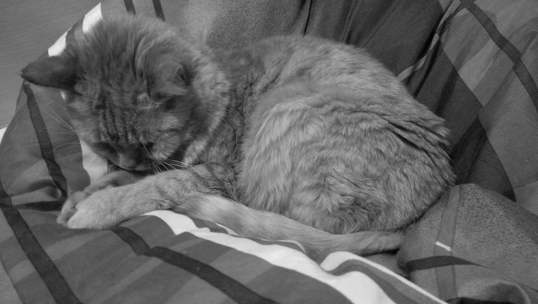
\includegraphics[width=\textwidth]{jerry_flt_20_0-001}
		\caption*{$\sigma_s = 20, \sigma_r = 0.001$}
	\end{subfigure}	
\caption{An image of Jerry. Applying the bilateral filter with a very small range value $\sigma_r$ does not have any effect.}
\label{fig:jerry_small_range}
\end{figure}

\begin{figure}[ht]
	\centering
	%\textbf{Title}\par\medskip
	\begin{subfigure}[h]{0.8\textwidth}
		\centering
		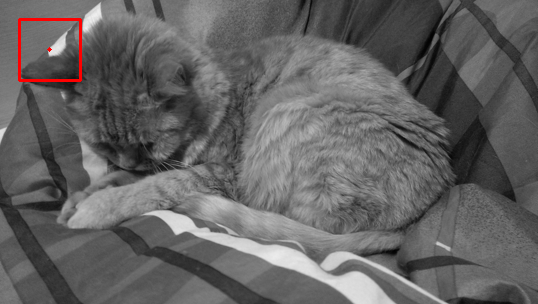
\includegraphics[width=\textwidth]{jerry_kernel_input}
		\caption*{Input image. Red: the pixel for which the filter kernels are visualized.}
	\end{subfigure}
	
	\vspace{2mm}
	\begin{subfigure}[h]{0.4\textwidth}
		\centering
		
\includegraphics[width=\textwidth]{jerry_kernel_spatial_20}
		\caption*{Spatial filter kernel, $\sigma_s = 20$}
	\end{subfigure}
	~ 
	\begin{subfigure}[h]{0.4\textwidth}
		\centering
		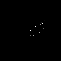
\includegraphics[width=\textwidth]{jerry_kernel_range_0-001}
		\caption*{Range filter kernel, $\sigma_r = 0.001$}
	\end{subfigure}	
	
	\vspace{2mm}
	\begin{subfigure}[h]{0.4\textwidth}
		\centering
		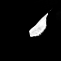
\includegraphics[width=\textwidth]{jerry_kernel_range_0-1}
		\caption*{Range filter kernel, $\sigma_r = 0.1$}
	\end{subfigure}
	~ 
	\begin{subfigure}[h]{0.4\textwidth}
		\centering
		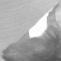
\includegraphics[width=\textwidth]{jerry_kernel_range_0-5}
		\caption*{Range filter kernel, $\sigma_r = 0.5$}
	\end{subfigure}
\caption{Visualized filter kernels for the pixel marked in red. A very low value for $\sigma_r$ causes the values of the range filter kernel to be very low almost everywhere -- higher values allow averaging of pixels that are less similar.}
\label{fig:kernel_small_range}
\end{figure}

\begin{figure}[ht]
	\centering
	%\textbf{Title}\par\medskip
	\begin{subfigure}[h]{0.48\textwidth}
		\centering
		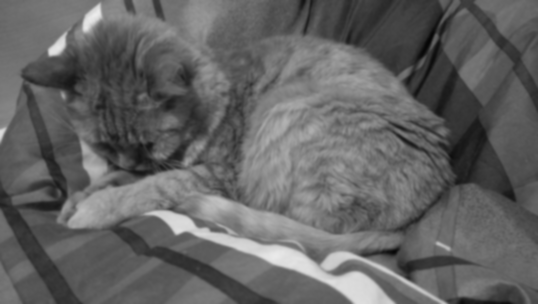
\includegraphics[width=\textwidth]{jerry_flt_1_2}
		\caption*{$\sigma_s = 1, \sigma_r = 2$}
	\end{subfigure}
	~ 
	\begin{subfigure}[h]{0.48\textwidth}
		\centering
		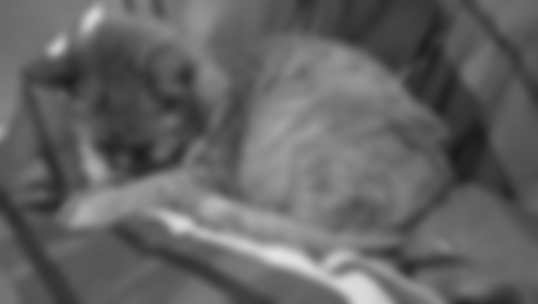
\includegraphics[width=\textwidth]{jerry_flt_5_2}
		\caption*{$\sigma_s = 5, \sigma_r = 2$}
	\end{subfigure}	
	
	\vspace{2mm}
	\begin{subfigure}[h]{0.48\textwidth}
		\centering
		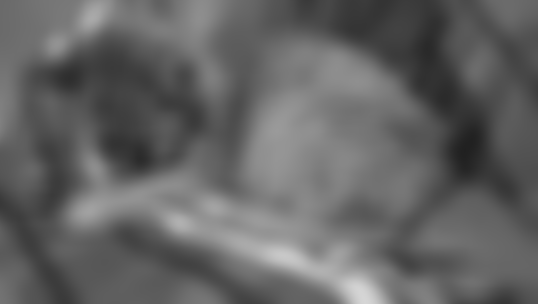
\includegraphics[width=\textwidth]{jerry_flt_10_2}
		\caption*{$\sigma_s = 10, \sigma_r = 2$}
	\end{subfigure}
	~ 
	\begin{subfigure}[h]{0.48\textwidth}
		\centering
		
\includegraphics[width=\textwidth]{jerry_flt_20_2}
		\caption*{$\sigma_s = 20, \sigma_r = 2$}
	\end{subfigure}
\caption{With a large value of $\sigma_r = 2$, the bilateral filter is pretty much just a Gaussian filter.}
\label{fig:jerry_large_range}
\end{figure}

\begin{figure}[ht]
	\centering
	%\textbf{Title}\par\medskip
	\begin{subfigure}[h]{0.48\textwidth}
		\centering
		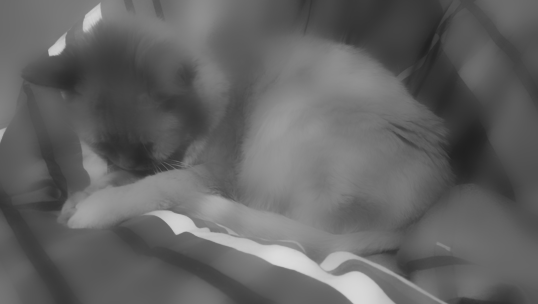
\includegraphics[width=\textwidth]{jerry_flt_10_0-2}
		\caption*{$\sigma_s = 10, \sigma_r = 0.2$}
	\end{subfigure}
	~ 
	\begin{subfigure}[h]{0.48\textwidth}
		\centering
		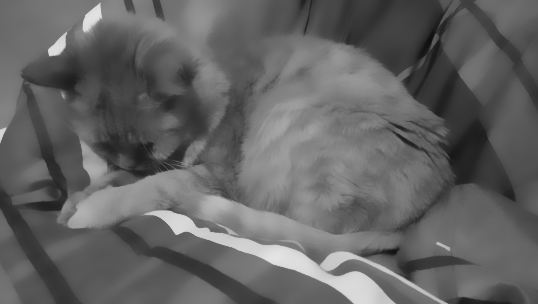
\includegraphics[width=\textwidth]{jerry_flt_5_0-1}
		\caption*{$\sigma_s = 5, \sigma_r = 0.1$}
	\end{subfigure}	
	
	\vspace{2mm}
	\begin{subfigure}[h]{0.48\textwidth}
		\centering
		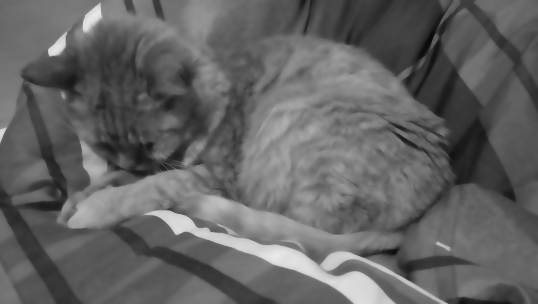
\includegraphics[width=\textwidth]{jerry_flt_2_0-12}
		\caption*{$\sigma_s = 2, \sigma_r = 0.12$}
	\end{subfigure}
	~ 
	\begin{subfigure}[h]{0.48\textwidth}
		\centering
		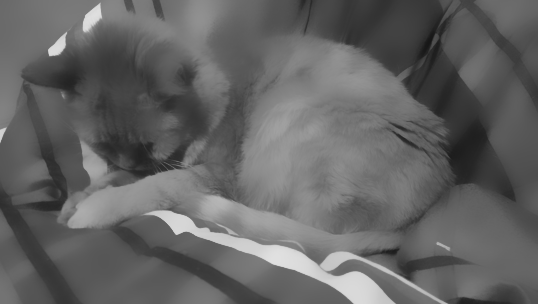
\includegraphics[width=\textwidth]{jerry_flt_8_0-12}
		\caption*{$\sigma_s = 8, \sigma_r = 0.12$}
	\end{subfigure}
\caption{Suitable values for $\sigma_s$ and $\sigma_r$ allow smoothing while preserving strong edges. However, sometimes it's difficult to find appropriate values such that all the edges are captured by the range kernel. This may lead to artifacts (blurred regions even though there would be edges), which is visible above at Jerry's neck.}
\label{fig:edge-preserving-smoothing}
\end{figure}

\subsection*{Tonemapping -- Bilateral vs. Gaussian Filter}
\todo{Text and comparisons go here!}
\end{document}